\chapter{Projektmonitoring}
\label{projektmonitoring}

\section{Projektverlauf}
In Abbildung \ref{overall_stories_gantt_chart} sind alle erledigten Stories mit Start- und Endpunkt auf der Zeitachse abgebildet. Leider werden die Sprints etwas verfälscht dargestellt, da wir einzelne bereits begonnene Stories aus Zeitgründen von einem Sprint in den nächsten verschoben haben (Stories \#25, \#113 und \#186). Diese werden von Redmine dann über mehrere Sprints hinweg dargestellt, was natürlich auch den Sprint künstlich "`verlängert"'.

\begin{figure}[H]
	\centering
	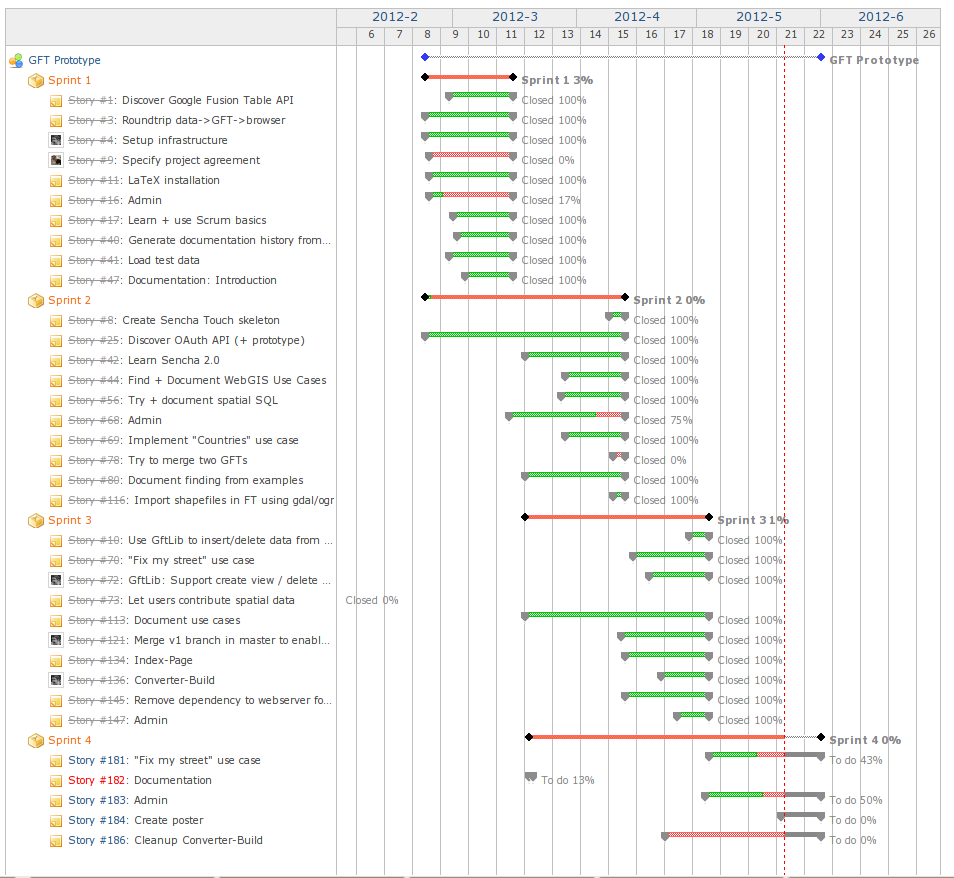
\includegraphics[width=\textwidth]{images/projektmanagement/overall_stories_gantt_chart}
	\caption{Gantt-Diagramm des Projektverlaufs}
	\label{overall_stories_gantt_chart}
\end{figure}

\section{Arbeitsaufwand}
Wie schon im Kapitel \ref{projektmanagement} beschrieben, war der vom Modul vorgegebene Aufwand pro Person auf \emph{240 Stunden} festgelegt. Wie in der Tabelle \ref{projektmanagement-arbeitsaufwand} ersichtlich haben wir diese Vorgabe beide leicht überschritten.

\begin{longtable}{|l|l|}
\hline 
\textbf{Person} & \textbf{Aufwand} \\ 
\hline 
Stefan Oderbolz & 255h \\ 
\hline 
Jürg Hunziker & 264h \\ 
\hline 
\caption{Arbeitsaufwand pro Person}
\label{projektmanagement-arbeitsaufwand}
\end{longtable} 

\section{Fazit}
Wir haben bezüglich Projektmanagement in diesem Projekt gute Erfahrungen mit Scrum sammeln können. Zuvor kannten wir beide diese Methodik mehr aus der Theorie, jetzt konnten wir die Stärken und Schwächen selbst kennenlernen. Es ist klar, dass wir Scrum für unsere Bedürfnisse etwas anpassen mussten, gerade weil wir nur zwei Personen im Projektteam waren. Es hat sich bewährt jeweils Stories für neue Features im Backlog zu erfassen, wenn diese gerade aufgetaucht sind. Bei der Planung eines neuen Sprints konnten wir so die bestehenden Stories mit Schätzungen versehen und diese dann auf den Sprint planen.

Dank unserem Tooling mit Redmine hatten wir stets den Überblick über unser Projekt und die noch offenen Stories bzw. deren Tasks. Dort konnten wir auch gleich unsere Zeiterfassung unterbringen, indem wir unsere Aufwände auf die Tasks buchen konnten. Das Projekt war hingegen fast zu kurz, um von den Stories Points zu profitieren. Wir haben über alle 4 Sprints hinweg mit durchschnittlich 12 Points pro Sprint gerechnet.